This chapter describes how the simulation is implemented in detail.
The development of the simulation has been done in Matlab.
The first part of the chapter mainly discusses the sensor model implementations while the second part is about the implementation of the state estimator itself.

\section{Sensor Models}
How the concept of the different sensor models work is described in chapter \ref{ch:Approach}.
In the following the implementation which is used in the simulation will be described in detail.
First in general for all sensors, followed by the different characteristics of each sensor.

\subsection{Perfect Sensor}
To calculate the prefect sensor data the trajectory is put into the equations which were defined before.
In Figure \ref{fig:GeneratedPerfectSensor} those generated sensor data as well as the trajectory used for this can be seen.

\begin{figure}[h!]
 \centering
 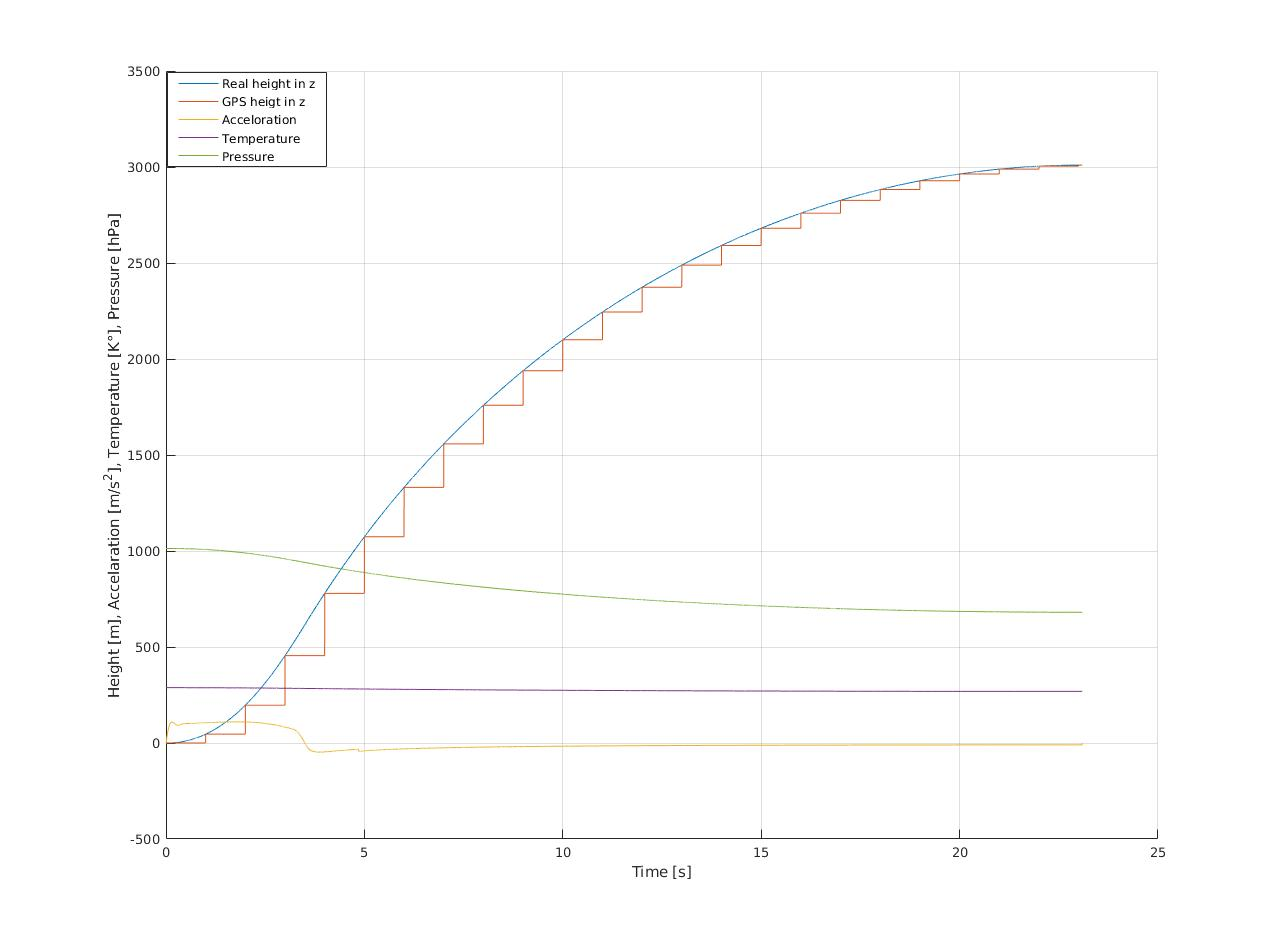
\includegraphics[width=0.8\textwidth]{./Pictures/GeneratedSensorData.jpg}
 % GeneratedSensorData.jpg: 0x0 pixel, 300dpi, 0.00x0.00 cm, bb=
 \caption{Generated sensor data}
 \label{fig:GeneratedPerfectSensor}
\end{figure}

\newpage
\subsubsection{Accelorometer}
Due to the fact that the whole simulation works with discrete time stamps the derivative of the height can not be done formally.
So it is done by calculating the difference between each data point to the next and then weighting those by the delta in time between them.
This has to be done two times to get from the height to the acceleration.
The unit for the acceleration in this simulation is meters per second squared.

\subsubsection{Gyrometer}
As stated before the pitch angle can not be directly generated.
But as can be seen from the data of the test flights the angle stays more or less the same wile the motor is burning.
This make sense because during this time the main acceleration comes from one determined direction and stabilises the rocket.
After the burnout the pitch angle does change more or less randomly depending on strength and direction of the wind that hits the rocket.
To simulate this the values are generated randomly and then low pass filtered with a moving average filter to represent that behaviour.
While doing this the random values are kept small during the burning of the motor and raised afterwards to higher values.

\subsubsection{Barometer}
The measurements from the barometers are depending on the atmospheric model which is used in this simulation.
For reasons of simplicity the start pressure is chosen as the mean pressure at sea level which is 1013.35 hP.
Also the temperature at the beginning is chosen as 288.15 Kelvin (15 °C) which also represents the mean value on the sea level.
Last but not least the temperature gradient is chosen as - 0.0065 K/m, which is a commonly used value.
For the state estimation in a test flight those values have to be determined before the start, especially the temperature gradient.

Since the barometers do sample at 100 Hz the measurements have to be down sampled.
As with the GPS sensor below this is achieved by a zero order hold conversion instead of direct down sampling

\subsubsection{GPS}
As stated in chapter \ref{ch:Approach} the GPS signal is just the height with a different sampling time.
To maintain the vectors length which simplifies the later use in the estimation algorithm,
the signal is acquired with a zero order hold conversion instead of a down sampling.

%@ToDo: Add code for the zero order hold convertion

\subsection{Noise}
To generate the noise out of the data from the test flight, it has first to be extracted.
It is assumed that the noise of the data is different depending on the state of the rocket (before ignition, during motor burning, after burnout untill parachute ejection),
but it should have more or less the same properties between those events.
Based on this, the data vector has to be separated in those different sections first.
For this the accelerometer measurements are iterated to find the time stamps on which those events happen, as can be seen in Figure \ref{fig:AccelerationMarks}.


\begin{figure}[h!]
 \centering
 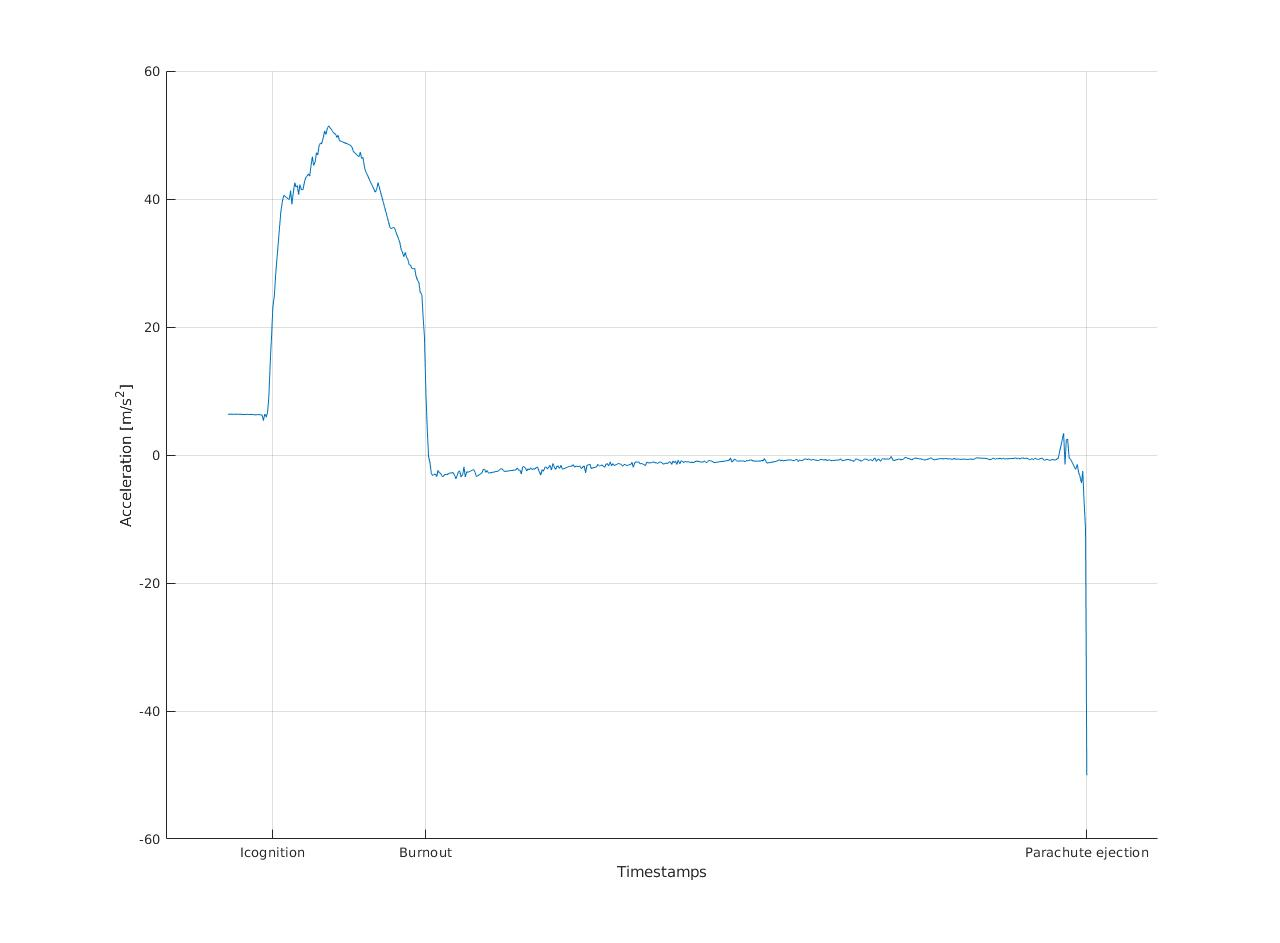
\includegraphics[width=0.8\textwidth]{./Pictures/AccelerationMarks.jpg}
 % AccelerationMarks.pdf: 0x0 pixel, 300dpi, 0.00x0.00 cm, bb=
 \caption{Timestamps drawn out of acceleration measurements}
 \label{fig:AccelerationMarks}
\end{figure}


If done so, polynomials of the order two are fitted on this measurements with the least squared error method.
Those polynominals represent the functions / the values which are assumed to be the noiseless data with possible offsets.
So if now these polynominals are subtracted from the test flight data the result are the measurements with zero mean.
From this point on this noise can be examined on its parameters, like the power density, the probability distribution and the variance, as can be seen in Figure \ref{fig:PF_AC_HIST_Accel}.

%% pictue of autocorrelation, histogramm etc from sensor data noise
\begin{figure}[h!]
 \centering
 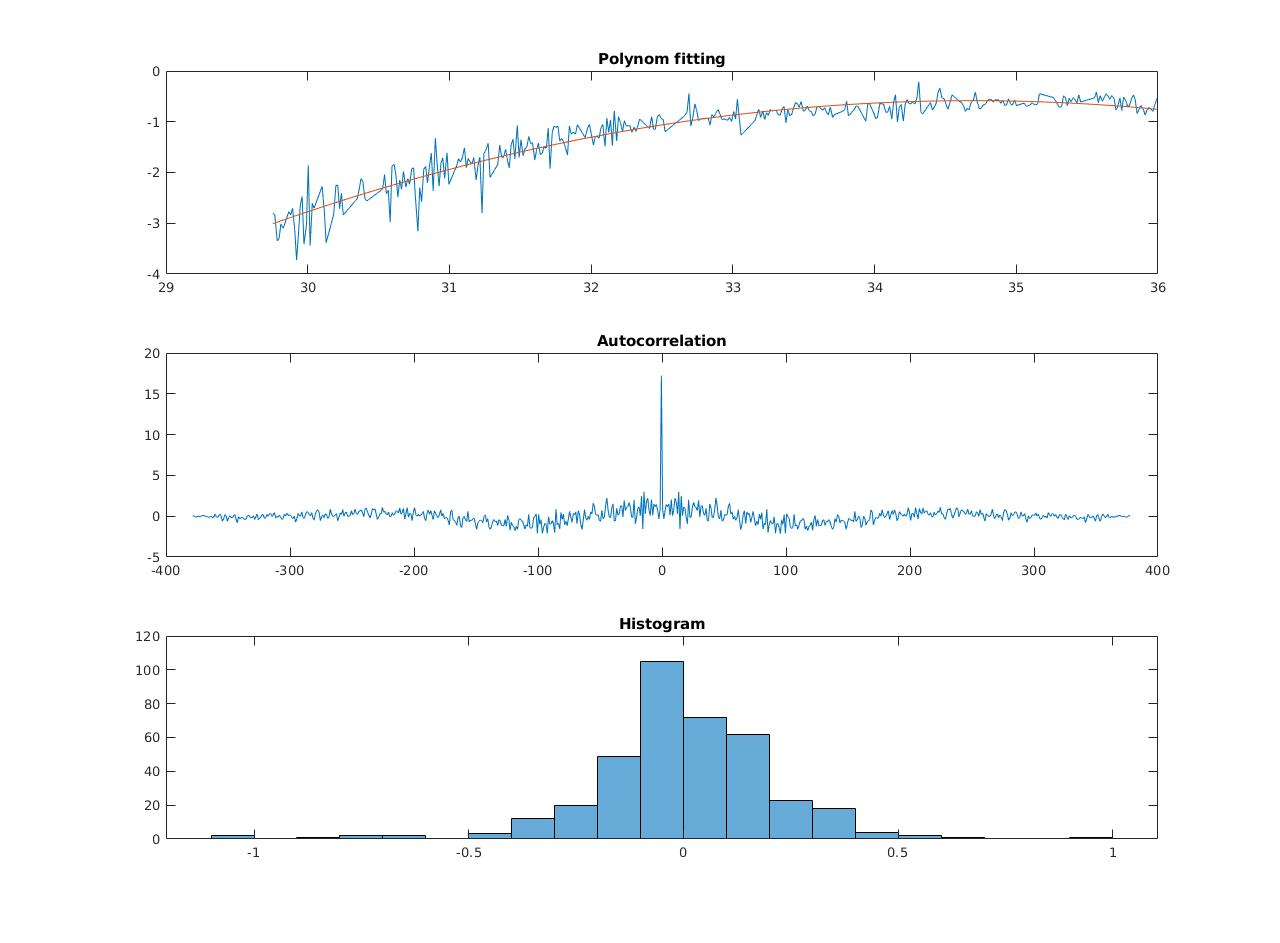
\includegraphics[width=0.8\textwidth]{./Pictures/PF_AC_HIST_Accel.jpg}
 % PF_AC_HIST_Accel.jpg: 0x0 pixel, 300dpi, 0.00x0.00 cm, bb=
 \caption{Polyfit Autoccorellation and Histogramm}
 \label{fig:PF_AC_HIST_Accel}
\end{figure}


This noise data can now be used to solve the Yule Walker Equation to get an AR model.
For this the aryule() function can be used which estimates an AR model of the order N as well as the variance directly out of the noise vector.
To achieve this it estimates the autocorrelation out of the given noise vector.
For the best possible results the corresponding data from all test flights were put together and used as one great noise vector.
Before doing this, the data had to be resampled so that the AR models can be properly used in the simulation.
With those AR models, the noise can be regenerated by filtering white noise with the correct variance.
This generated noise can now be compared to the noise from the test flight data.

%% picture of pwelch plot from both noise vectors
\begin{figure}[h!]
 \centering
 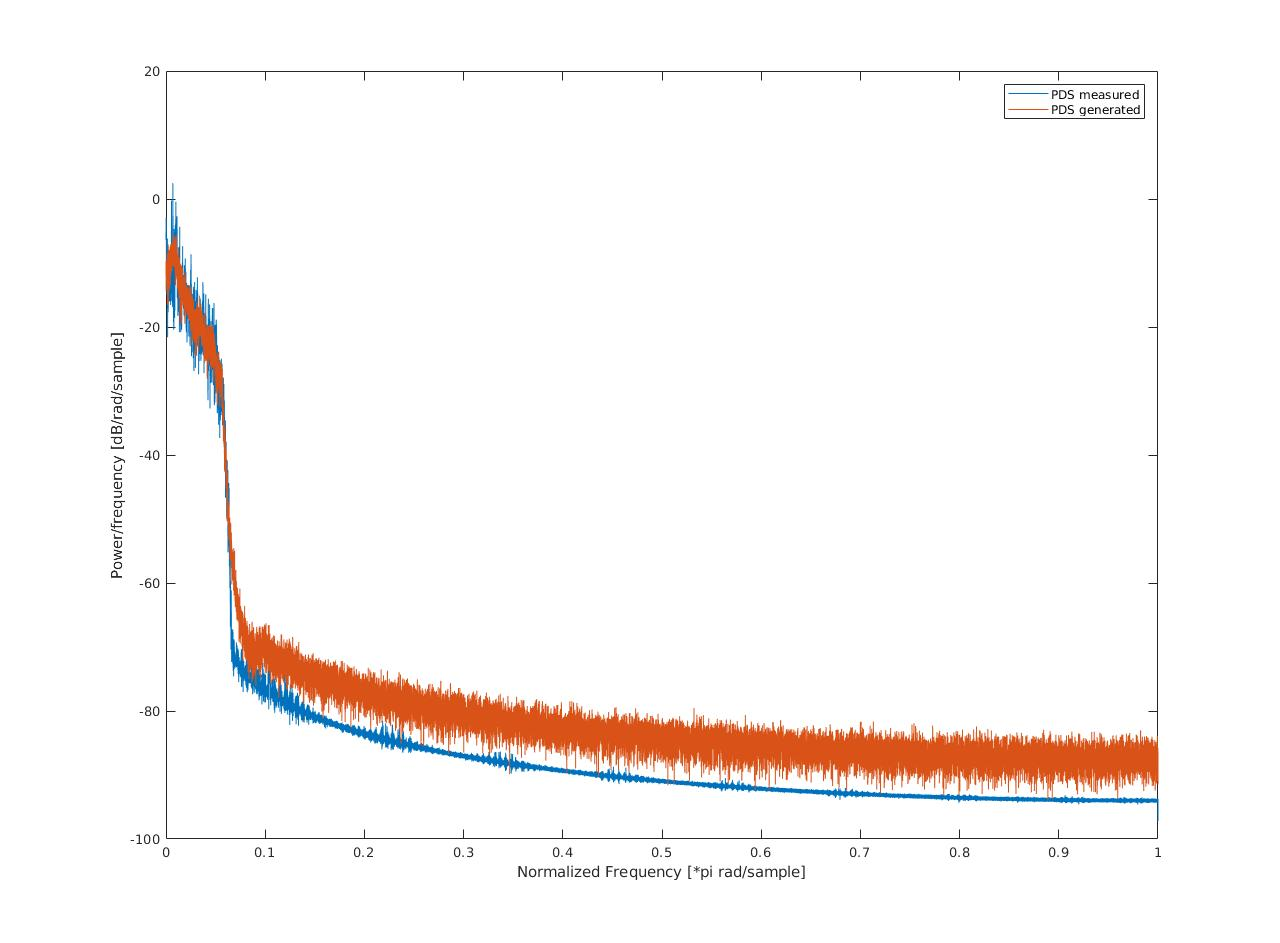
\includegraphics[width=0.8\textwidth]{./Pictures/PDSnoise.jpg}
 % PDSnoise.jpg: 0x0 pixel, 300dpi, 0.00x0.00 cm, bb=
 \caption{PDS from the measured and generated noise}
 \label{fig:PDSNoise}
\end{figure}


As can be seen in figure \ref{fig:PDSNoise} both noises resemble each other in their power density spectrum much more than the white noise would.
So this AR model is exported to the simulation script and can be used there to generate the real sensor data.

\subsubsection{Accelorometer}
The noise which is on the accelorometer is special because it often has a drift which results in a more or less constant offset.
To recreate this, the offset can be estimated from the test flight data.
Especially the data before the ignition is helpful, because the value that should be measured is known.

\subsubsection{Gyrometer}
For the gyrometer noise a separate script has been written to calculate the proper pitch angle and filter out the offset before generating the AR model.
This because the gyrometer measurements which are available are in degrees per second
and have therefore to be integrated before they resemble the correct pitch angle.
In addition to this it is complicated to define which part of the measurements are noise and which is the ground truth.
It was found that the estimated AR model could not regenerate noise with the same characteristics.
Because of that, the noise has to be low pass filtered another time to resemble the real noises better.
For this task an IIR filter of order 200 was found best.
With this also the Gyrometer measurements could be properly handled.

\subsubsection{Barometer}
The barometer noise itself has no real capacities which were not already discussed before.

\subsubsection{GPS}
The GPS noise capacities were only found with measurements that were taken for a longer time period while the GPS receiver stayed at the same place.
So based on the assumption that the GPS measurements are independent from the motor vibrations and the rocket posture changes the noise will have the same capacity over the whole flight.
This should be suitable as long as the receiver does not lose its fix.

\newpage
\subsection{Real Sensor}
To now generate the real sensor data, the different noises have to be generated with the calculated AR models and added to the perfect sensor data.
For this a vector of normal distributed random values is generated and multiplied by the square root of the corresponding variance (hence the standard deviation).
This white noise is now filtered by the corresponding AR-model and can then be added onto the corresponding perfect sensor data, which results in the real sensor data.

\subsubsection{Accelorometer}
\begin{figure}[h!]
 \centering
 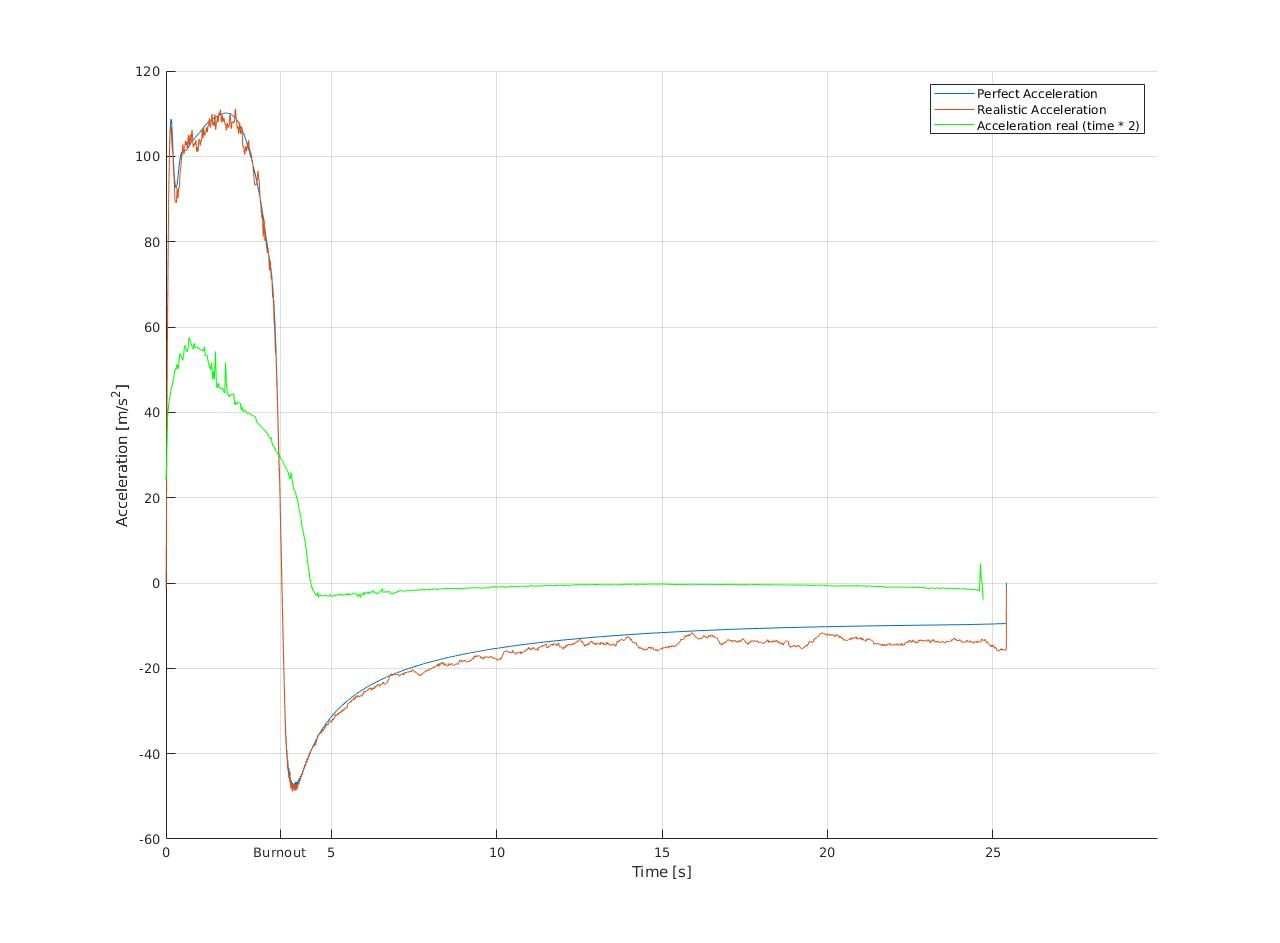
\includegraphics[width=0.8\textwidth]{./Pictures/AccelPerfVSReal.jpg}
 % AccelPerfVSReal.jpg: 0x0 pixel, 300dpi, 0.00x0.00 cm, bb=
 \caption{Plot of perfect acceleration vs realistic vs measured}
 \label{fig:AccelPerfVsReal}
\end{figure}
In Figure \ref{fig:AccelPerfVsReal} the different generated values as well as the data from a test flight can be seen.
The time vector from the test flight was stretched by the factor two to make the observation easier.
Also it has to be said that the test flight was with a smaller rocket which flew only at an apogee of around 300 meters.
This explains why the acceleration is not as great as in the generated data and why the time vector had to be stretched.
But the plot shows that the noise as well as the perfect data resemble the acceleration from the test flight in a appropriate way.

\newpage
\subsubsection{Gyrometer}
\begin{figure}[h!]
 \centering
 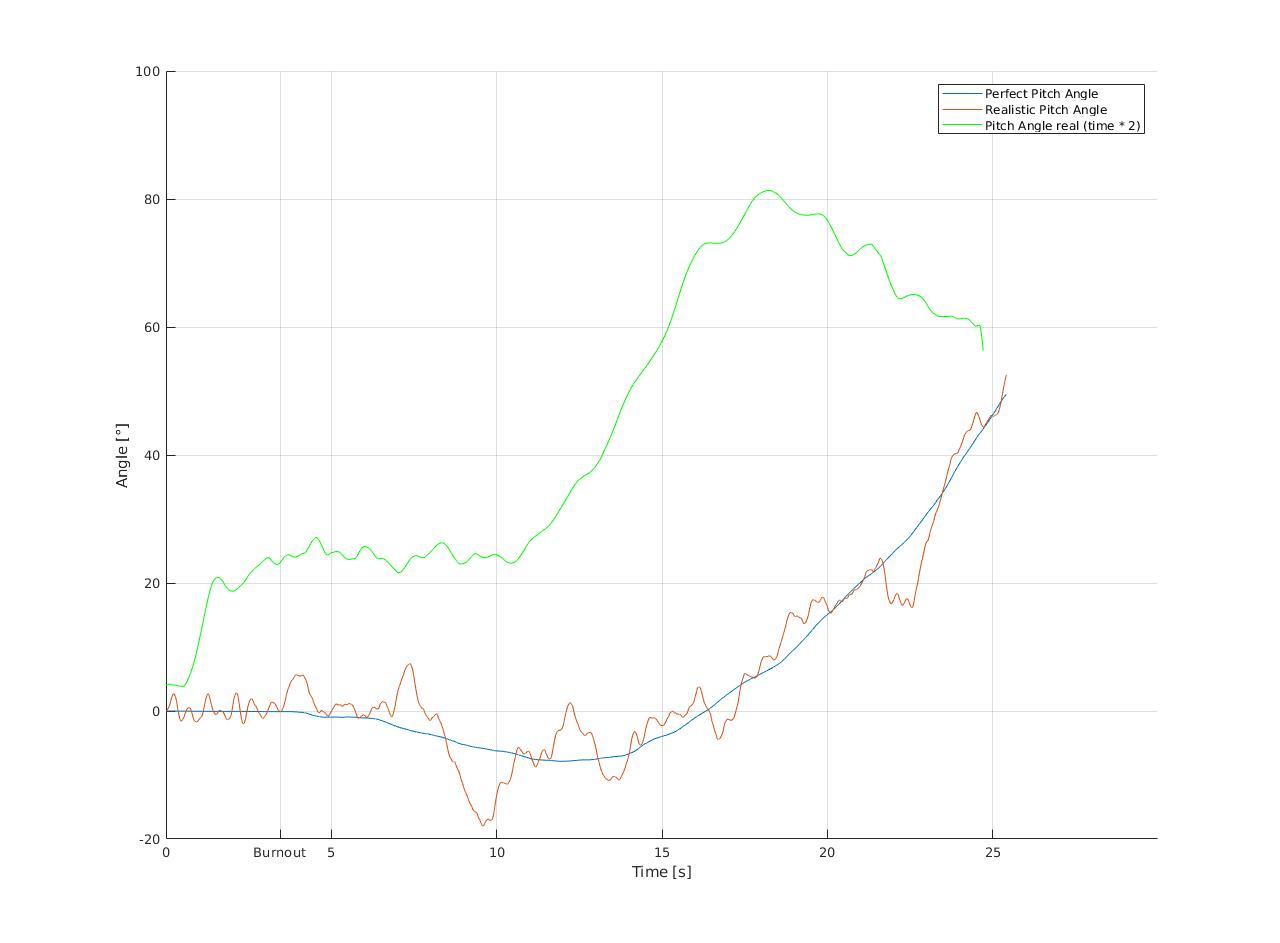
\includegraphics[width=0.8\textwidth]{./Pictures/PitchPerfVSReal.jpg}
 % PitchPerfVSReal.jpg: 0x0 pixel, 300dpi, 0.00x0.00 cm, bb=
 \caption{Plot of perfect gyrometer vs realistic vs measured}
 \label{fig:PtichPerVSReal}
\end{figure}
Figure \ref{fig:PtichPerVSReal} shows the generated gyrometer data.
Like in the acceleration plot the time vector from the test flight data was adjusted for better observability.
It should also be explained that due to the property of the pitch angle (more or less random depending on air current etc)
the generated realistic pitch angle must not resemble the measured angle in its specific value.
Important to show is that the noises have the same capacities which they do.
Also it can be seen that the assumption that the angle does not change much during the burning of the motor is appropriate despite a quick change at the start.

\newpage
\subsubsection{Barometer}
\begin{figure}[h!]
 \centering
 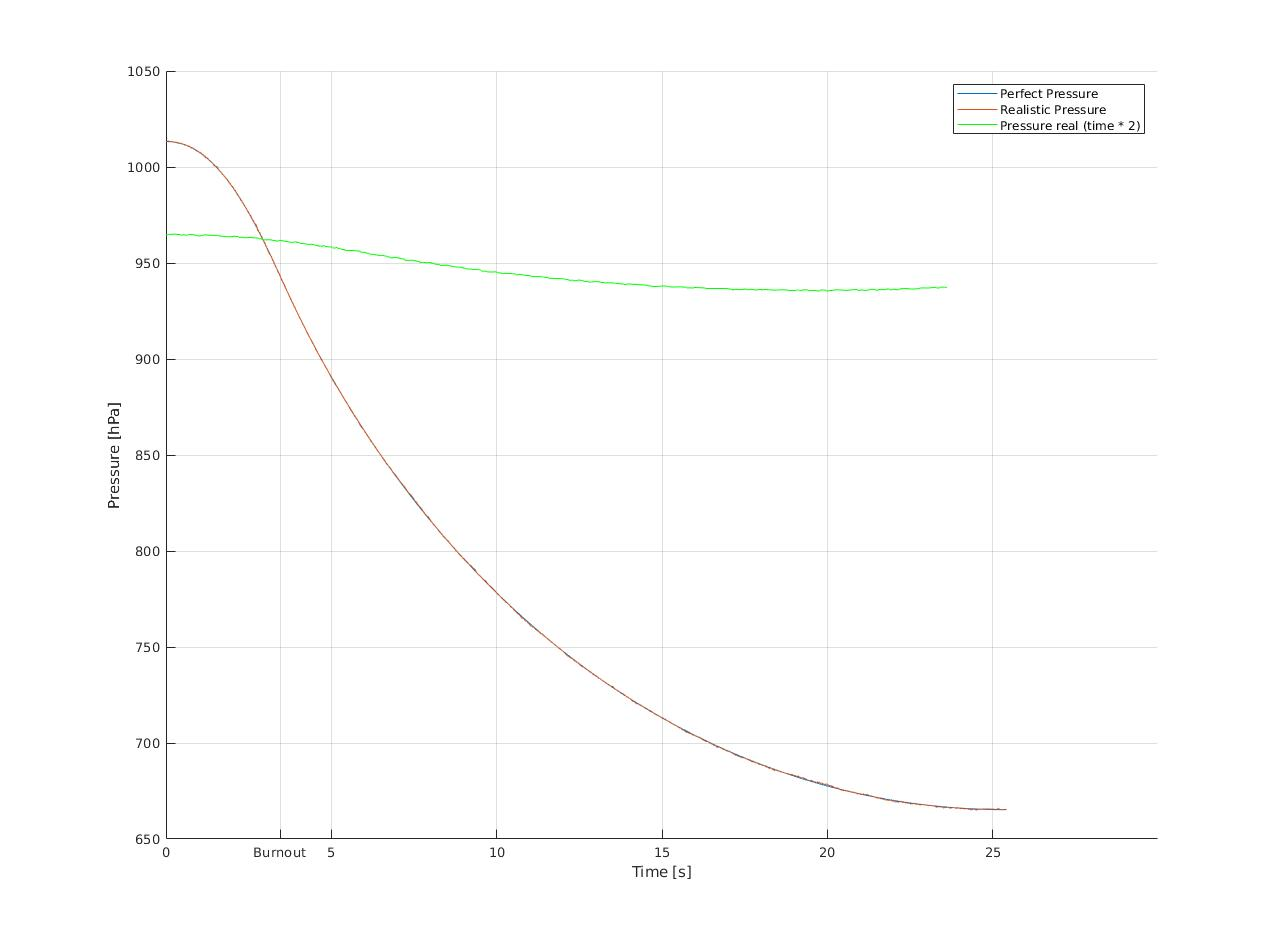
\includegraphics[width=0.8\textwidth]{./Pictures/PressurePerfVSReal.jpg}
 % PressurePerfVSReal.jpg: 0x0 pixel, 300dpi, 0.00x0.00 cm, bb=
 \caption{Plot of perfect barometer vs realistic vs measured}
 \label{fig:PressurePerfVSReal}
\end{figure}
The realistic pressure measurements from a barometer are shown in Figure \ref{fig:PressurePerfVSReal}.
The noise itself does not look as it would have a great impact on the perfect data.
But because the pressure does change by around 350 hP during the upflight and the noise is only around 1 to 3 hP it can not be seen that good.
The comparison with the real measured data (in the figure also with a stretched time vector) shows that the generated realistic measurement data does resemble the real measurements well.

\newpage
\subsubsection{GPS}
\begin{figure}[h!]
 \centering
 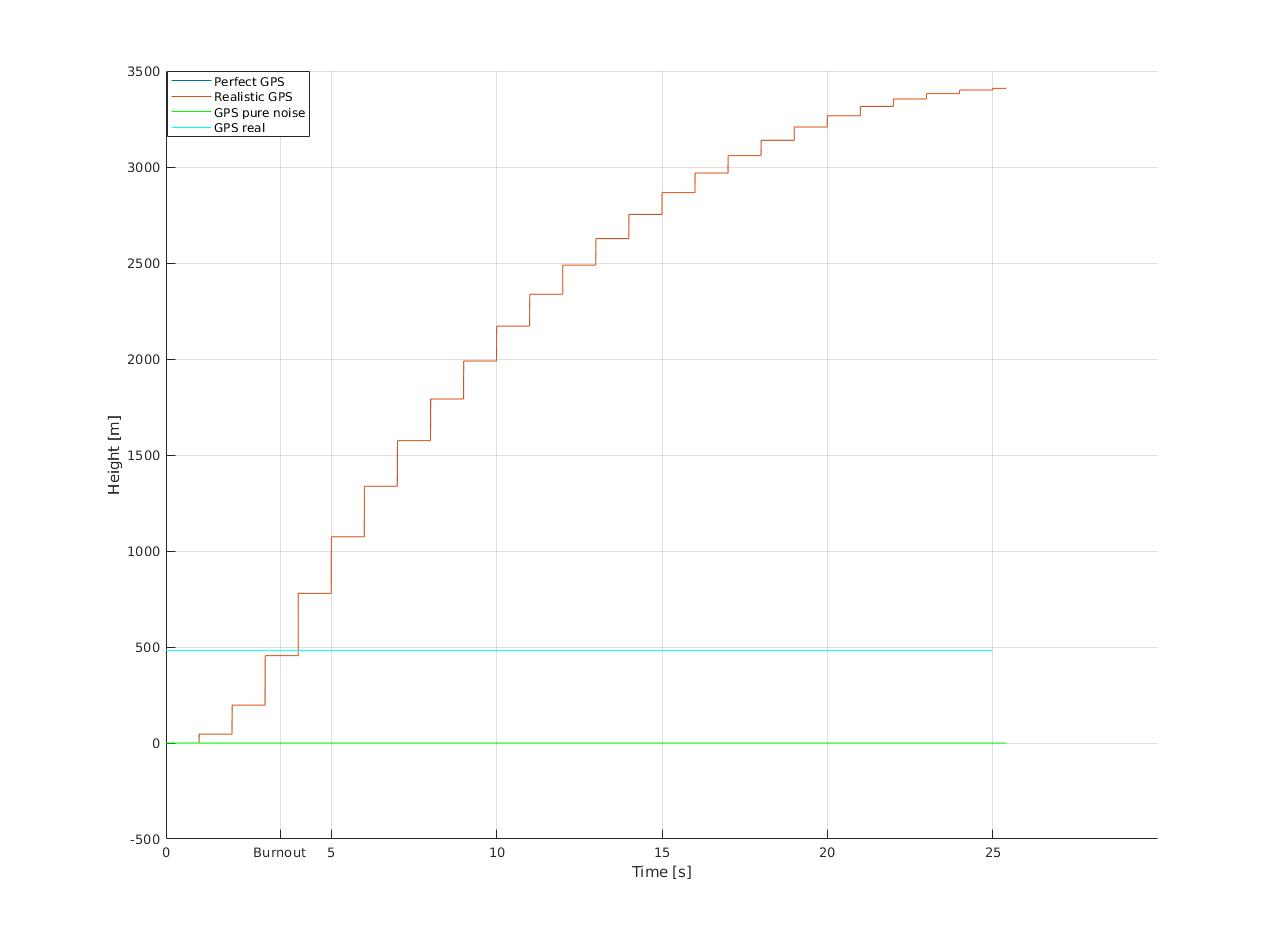
\includegraphics[width=0.8\textwidth]{./Pictures/GPSPerfVSReal.jpg}
 % GPSPerfVSReal.jpg: 0x0 pixel, 300dpi, 0.00x0.00 cm, bb=
 \caption{Plot of perfect GPS vs realistic vs measured}
 \label{fig:GPSPerfVSReal}
\end{figure}
Last but not least the generated GPS measurements can be observed in Figure \ref{fig:GPSPerfVSReal}.
In this plot the pure generated noise was also plotted because this way it can be best shown that it has real slow properties.
For comparison the measurements which were taken from a fixed position are plotted (because there were no usable GPS data from a test flight avaiable during the term of this thesis).
It can be seen that the test data does also resemble the noise from the generated data.


\section{State Estimation}
As stated in the last chapter the to be used state estimator is a discrete Kalman filter with dynamic noises on the measurements as well as on the system.
For this the noise matrices as well as the used loop is described below.

\subsection{System Model}
Based on the models stated in chapter \ref{ch:Approach} several different implementations can be derived.
For this simulation 8 models were implemented with each different capabilities.
To find the best suiting model all of them have been tested. The test results are discussed and evaluated in the next chapter.
\subsection{Adjustment}
Taking into account the noise characteristics of the measurements stated above, some adaptions to the model presented in chapter \ref{ch:Approach} have been made, which should hopefully result in better results.
\subsubsection{Offset}
The main adjustment is the inclusion of acceleration offset into the state vector.
This is a common tactic to minimise the impact of the offset. This works because by adding the offset to the state vector the state estimator can also estimate the actual offset which can then be used to correct the offset value \cite{DavidWSchultz2004}.
Therefore the state vector of a point mass would look like this.
$$ x = \begin{bmatrix}
        h_z \\
        v_u \\
        a_z \\
        a_{offset} \\
       \end{bmatrix}
$$
While the dynamic matrices A and B would stay the same apart from an additional dimension of zeros for the acceleration offset state variable.
\begin{align*}
 A = \begin{bmatrix}
      0 & 1 & 0 & 0 \\
      0 & 0 & 1 & 0 \\
      0 & 0 & 0 & 0 \\
      0 & 0 & 0 & 0
     \end{bmatrix}
     & \hspace{1cm}
 B = \begin{bmatrix}
      0 \\
      0 \\
      0 \\
      0
     \end{bmatrix}
\end{align*}
The y vector would stay the same while the output matrix $C^T$ will be adjusted so that both acceleration and acceleration offset in the state vector are added into the accelerometer measurements.
\begin{align*}
 y = \begin{bmatrix}
      h_{GPS} \\
      h_{p1} \\
      h_{p2} \\
      a
     \end{bmatrix}
     & \hspace{1cm}
 C^T = \begin{bmatrix}
      1 & 0 & 0 & 0 \\
      1 & 0 & 0 & 0 \\
      1 & 0 & 0 & 0 \\
      0 & 0 & 1 & 1
     \end{bmatrix}
\end{align*}

\subsubsection{Acceleration as Input}
An additional adjustment would be to consider the measured acceleration of the rocket as input into the system.
This should result into a system which could react faster to changes in the acceleration.
For this the measurement noise of the accelerometer would have to be placed in the system noise matrix
and therefore no additional system noise can be modulated.
For a point mass this would result in the following system matrices.
While the state vector and the A matrix would stay the same, the B vector would have to be adjusted like this.
$$ B = \begin{bmatrix}
        0 \\
        0 \\
        1
       \end{bmatrix}
$$
In addition the y vector would lose its acceleration measurements and the output matrix $C^T$ the corresponding dependencies.
\begin{align*}
 y = \begin{bmatrix}
      h_{GPS} \\
      h_{p1} \\
      h_{p2} \\
     \end{bmatrix}
      & \hspace{1cm}
 C^T = \begin{bmatrix}
        1 & 0 & 0 \\
        1 & 0 & 0 \\
        1 & 0 & 0 \\
       \end{bmatrix}
\end{align*}

\subsection{Measurement Noise}
The matrix on each time stamp for the measurement noise is rather easy to get in the simulation because the perfect measurements are known.

First the variance over the burning of the motor as well as over the up flight is calculated separately.
After that those values are used to generate a noise vector for each measurement.
In addition the implementation of the noise vector has the same length as all other used vectors.
These noise measurements are then concatenated into diagonal noise matrices as shown in the listing below:

\begin{lstlisting}[caption={Mesurements noise matrix conagonating}]
R_dyn = [GPSvar;ACLvar;HBM1var;HBM2var];         %Add the noise vectors into one matrix
R_dyn_m = diag(R_dyn(:,1)');                     %Make a diagonal first diagonal matrix
for n = 2:length(TimeVec)
    R_dyn_m = cat(3,R_dyn_m,diag(R_dyn(:,n)'));  %Concatogenate all noise vectors
end
\end{lstlisting}


If the noise matrix is displayed as a diagonal matrix,
it takes into account the assumption that the noises from the measurements are independent from each other.
This assumption can be made because of the fact that each measurement except those from the barometer (pressure and temperature) are made from different sensors.
Due to the fact that the temperature is not used for the state estimation, the measurements matrix can still be assumed as diagonal.

\subsubsection{Different Sampling Times}
In addition the measurement noise matrix can be used to adjust for the different sampling times of the sensors.
This is used for the barometers as well as the GPS sensors which are sampled slower as the state estimation itself loops.
This adjustment is achieved by maxing out (setting to the highest possible value) the corresponding variance in the measurement noise matrix R if no actual measurements are available.
As it can be seen in the formula to calculate the Kalman gain K,
$$  K = P\cdot C^T\cdot (C\cdot P\cdot C^T + R)^{-1} $$
maximum values in the R matrix result in nearly zero values in the corresponding K matrix.
Those near or exactly zero values result in ignoring the corresponding measurements from the y vector as can be seen in the measurement update equation.
$$  x = \hat{x} + K\cdot(y[k] - C^T \cdot \hat{x}) $$

With this vectors with the same length as the other vectors in the state estimation can be generated out of the measurements.
When implementing in an embedded system this can simply be achieved with an ``if'' statement that switches the R matrix value to the normal variance if a measurement arrives.

\subsection{System Noise}
The system noise describes how uncertain the system model is in comparison to the real system.
For this each entry in the diagonal matrix resembles the variance of the noise on the corresponding state variable.
In other words the system noise describes how far away from the predicted value the actual value can get in the next loop iteration.
For the system noise the behaviour of the system during the flight has to be examined.
This can be done in different ways.
The first way would be to view the different ground truth curves of those state variables,
which do have system noise acting on them (acceleration, pitch angle, pressure if linearised).
\begin{figure}[h]
 \centering
 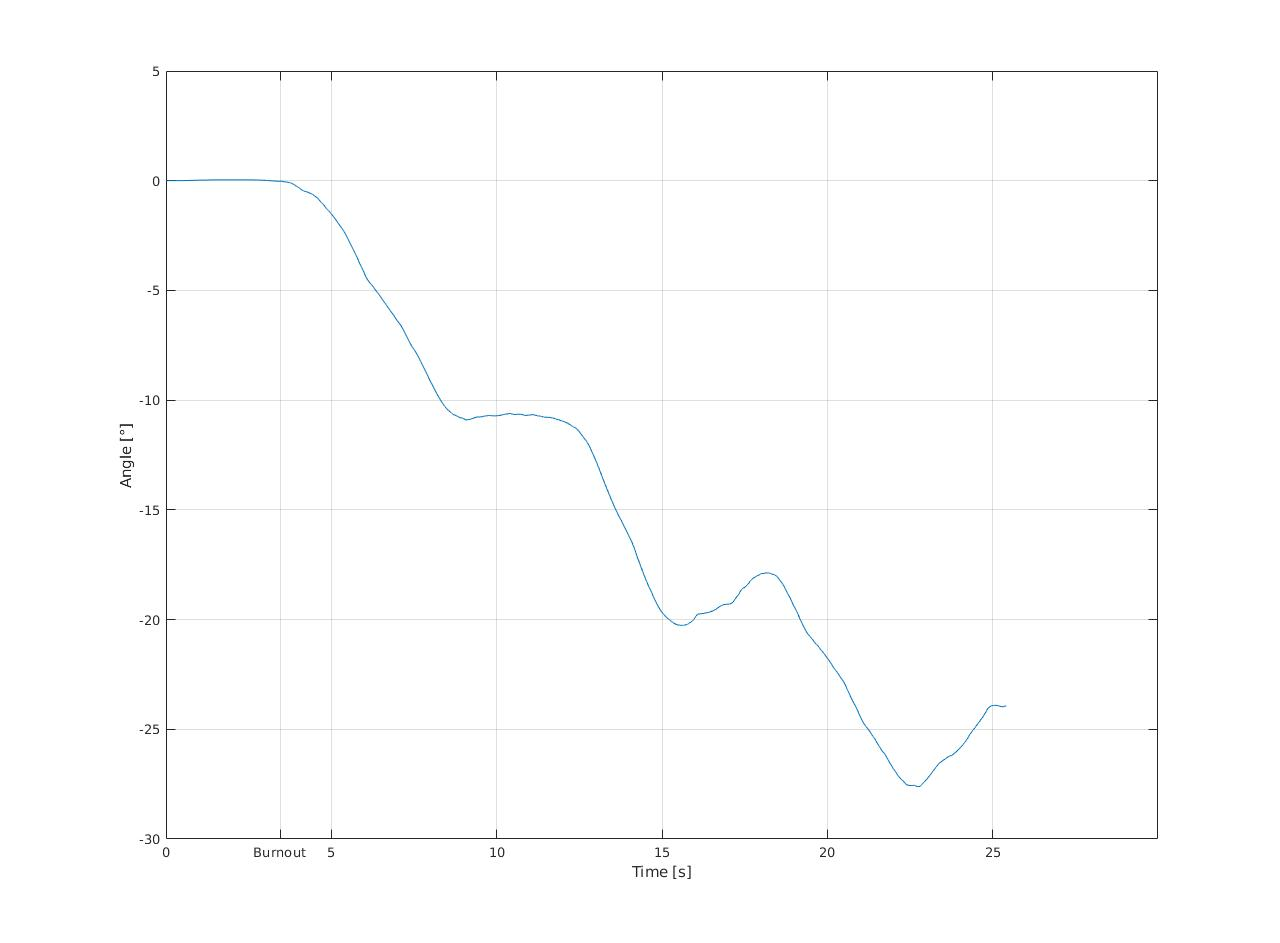
\includegraphics[width=.8\textwidth]{./Pictures/PitchAnglePlot.jpg}
 % PitchAnglePlot.jpg: 0x0 pixel, 300dpi, 0.00x0.00 cm, bb=
 \caption{Plot of pitch angle}
 \label{fig:PitchAnglePlot}
\end{figure}
For example Figure \ref{fig:PitchAnglePlot} shows the pitch angle.
In the system models there are no influences on this state value except for the measurements.
So to describe the changes of the value which are observed with the measurements a system noise has to have an impact on the pitch angle.
As it can be seen in the plot the angle does not change in a great manner until the burnout so the system noise till the burnout should also be rather small.
After the burnout the angle changes a lot more but keeps changing in the same way all over the time. \\

As a second attempt since the system noise describes the capability of the value to change over time independent from the dynamic system description
it can also be achieved by deviating the ground truth value vector.
For this the following matlab code can be used.
\begin{lstlisting}[caption={System noise generation with deviation}]
ACEL = abs(diff(a));                            % Deviating the gournd truth acceleration
ACEL = filter(ones(1,100)*1/100,1,ACEL);        % Low pass filtering
ACEL = [ACEL ACEL(end)];                        % Maintain vector length
\end{lstlisting}
This shows that after the deviation the absolute value from the deviation result is taken since a variance cannot or should not be negative.
After that the values are low pass filtered to make a more steady system noise description.

\subsection{Sensor Outfall}

An additional interesting scenario which can be observed with the simulation is the outfall of sensors.
This is needed to test the reliability requirements which states that the algorithm should still be working if 2-3 sensor fail, accepting that the estimation results will not be as accurate any more.
For this it has to be said that it has to be detected that a sensor fails to adjust the estimation algorithm.
If done so the variance can be adjusted for this sensor in the same way as stated above for the GPS signal by maxing its variance out.

It is achieved by a simple if statement which does exactly that if a sensor fail is recognised.

\subsection{Loop}
Finally the state estimation is implemented in a simple loop which iterates trough each given time stamp.
First the needed vectors and matrices have to be initialised with the right value.
In most system model versions the u vector remains zero while all measurements are brought into the estimation loop trough the y vector.
But there are some others where the acceleration and the pitch angle are brought into the estimation loop over the u vector only and the remaining measurements through the y vector.
That means that the current state vector x has to be initialised with the value of the corresponding sensors at the start,
which is presumably zero for all states except pressure and temperature.
The loop itself calculates the equations as they were stated in chapter \ref{ch:Approach}.

In addition if values from the measurements can not be transformed into the state vector values directly or only with a linearising calculation,
they have to be transformed first before entering the system.
For example pressure and temperature into height or acceleration and pitch angle into pure vertical acceleration.\\

Below is an example for the estimation loop for a rank five system. This model contains height, speed, acceleration, acceleration offset and pitch angle as state variables.
\begin{lstlisting}[caption={State Estimation Loop}]
% Initalzation
u = zeros(1,length(TimeVec));                       %Input vector is zero
y = [h_mes_GPS;a_mes;p_mes_1;p_mes_2;phi_mes];      %Output are the measurements
x = [0;0;0;0;0];                                    %Start Vector should be like this
P = eye(5);                                         %Standart can maybe be increased
Height1 = 0;
Height2 = 0;
Temp = T(1);
x_est_loop = zeros(size(x,1),length(TimeVec));     %Vector for the state estimation values

% Estimation loop
for k = 1:length(TimeVec)
    K = P*C'*pinv(C*P*C' + R_dyn_m(:,:,k));
    % Calculate height out of pressure measurements.
    Height1 = CalcHeight(Po,p_mes_1(k),Temp,0,true,TgradSimu); 
    Height2 = CalcHeight(Po,p_mes_2(k),Temp,0,true,TgradSimu);
    % Calculate the pure vertical acceleration with the pitch angle.
    acc = a_mes(k) * cos(x(5)*pi/180);		
    x = x + K*([h_mes_GPS(k);acc;Height1;Height2;phi_mes(k)] - C*x);
    P = (eye(5)-K*C)*P;

    x_est_loop(:,k) = x;                           %Save data from the Sensor fusion

    x = Ad*x + Bd*u(k);
    P = Ad*P*Ad' + Gd*Q_dyn_m(:,:,k)*Gd';
end
\end{lstlisting}

